%%%%%%%%%%%%%%%%%%%%%%%%%%%%%%%%%%%%%%%%%
% Large Colored Title Article
% LaTeX Template
% Version 1.1 (25/11/12)
%
% This template has been downloaded from:
% http://www.LaTeXTemplates.com
%
% Original author:
% Frits Wenneker (http://www.howtotex.com)
%
% License:
% CC BY-NC-SA 3.0 (http://creativecommons.org/licenses/by-nc-sa/3.0/)
%
%%%%%%%%%%%%%%%%%%%%%%%%%%%%%%%%%%%%%%%%%

%----------------------------------------------------------------------------------------
%	PACKAGES AND OTHER DOCUMENT CONFIGURATIONS
%----------------------------------------------------------------------------------------

\documentclass[DIV=calc, paper=a4, fontsize=11pt]{article}	 % A4 paper and 11pt font size
\usepackage[margin=1.0in]{geometry}

\usepackage{graphicx}
\usepackage[hidelinks]{hyperref}
\usepackage{lipsum} % Used for inserting dummy 'Lorem ipsum' text into the template
\usepackage[english]{babel} % English language/hyphenation
\usepackage[protrusion=true,expansion=true]{microtype} % Better typography
\usepackage{amsmath,amsfonts,amsthm} % Math packages
\usepackage[svgnames]{xcolor} % Enabling colors by their 'svgnames'
\usepackage[hang, small,labelfont=bf,up,textfont=it,up]{caption} % Custom captions under/above floats in tables or figures
\usepackage{booktabs} % Horizontal rules in tables
\usepackage{fix-cm}	 % Custom font sizes - used for the initial letter in the document
\usepackage{xspace}
\usepackage{float}
\restylefloat{table}

\usepackage{sectsty} % Enables custom section titles
\allsectionsfont{\usefont{OT1}{phv}{b}{n}} % Change the font of all section commands

\usepackage{fancyhdr} % Needed to define custom headers/footers
\pagestyle{fancy} % Enables the custom headers/footers
\usepackage{lastpage} % Used to determine the number of pages in the document (for "Page X of Total")

% Headers - all currently empty
\lhead{}
\chead{}
\rhead{}

\definecolor{davysgrey}{rgb}{0.33, 0.33, 0.33}

\newcommand \bulk {\textit{bulk\_extractor}\xspace}
\newcommand \viewer {\textbf{Bulk Extractor Viewer}\xspace}

% Footers
\lfoot{}
\cfoot{}
\rfoot{\footnotesize Page \thepage\ of \pageref{LastPage}} % "Page 1 of 2"

\renewcommand{\headrulewidth}{0.0pt} % No header rule
\renewcommand{\footrulewidth}{0.4pt} % Thin footer rule

\usepackage{lettrine} % Package to accentuate the first letter of the text
\newcommand{\initial}[1]{ % Defines the command and style for the first letter
\lettrine[lines=3,lhang=0.3,nindent=0em]{
\color{LightBlue}
{\textsf{#1}}}{}}

%----------------------------------------------------------------------------------------
%	TITLE SECTION
%----------------------------------------------------------------------------------------

\usepackage{titling} % Allows custom title configuration

\newcommand{\HorRule}{\color{LightBlue} \rule{\linewidth}{1pt}} % Defines the gold horizontal rule around the title

\pretitle{\vspace{-60pt} \begin{flushleft} \HorRule \fontsize{20}{20} \usefont{OT1}{phv}{b}{n} \color{davysgrey} \selectfont} % Horizontal rule before the title

\title{\bulk: A Triage Tool for Digital Forensics} % Your article title

\posttitle{\par\end{flushleft}\vskip 0.5em} % Whitespace under the title

\preauthor{\begin{flushleft}\large \lineskip 0.5em \usefont{OT1}{phv}{b}{sl} \color{davysgrey}} % Author font configuration

\author{Operations Concept} % Your name

\postauthor{\footnotesize \usefont{OT1}{phv}{m}{sl} \color{Black} % Configuration for the institution name
%University of California % Your institution

\par\end{flushleft}\HorRule} % Horizontal rule after the title

\date{\today} % Add a date here if you would like one to appear underneath the title block

%----------------------------------------------------------------------------------------

\begin{document}

\maketitle % Print the title

\thispagestyle{fancy} % Enabling the custom headers/footers for the first page 

%----------------------------------------------------------------------------------------
%	ABSTRACT
%----------------------------------------------------------------------------------------

% The first character should be within \initial{}
\initial{M}\textbf{any of today's digital forensic tools were created for finding evidence where the possession of evidence is the  crime itself (such as in a child pornography case). This paradigm can be effective in the law enforcement context but is not especially useful for cyber-defense and investigative purposes. Instead, forensic tools must be designed to facilitate investigation and exploration rather than simply evidence identification\cite{Next10Years}. \bulk solves this problem by providing all the necessary capabilites to help examiners find specific pieces of evidence and to assist in investigations.}

%----------------------------------------------------------------------------------------
%	ARTICLE CONTENTS
%----------------------------------------------------------------------------------------
\section*{What does it do?}
\bulk is a digital forensics system that extracts information. Given a disk image, directory of files, network or cell phone data, \bulk scans data thoroughly, decompresses when necessary, discovers features and carves objects (Figure~\ref{fig:highLevelBulk}). The features extracted by \bulk include email addresses, credit card numbers, URLs, executables, and JPEGs, and other data types.\\

\noindent
\bulk complements existing forensic tools  by providing output that facilitates data exploration, triage and investigation. Users can search the output for specific terms and ideas; they can also browse the groups of features by frequency and quickly find salient data that can guide the early stage of investigations.

\begin{center}
  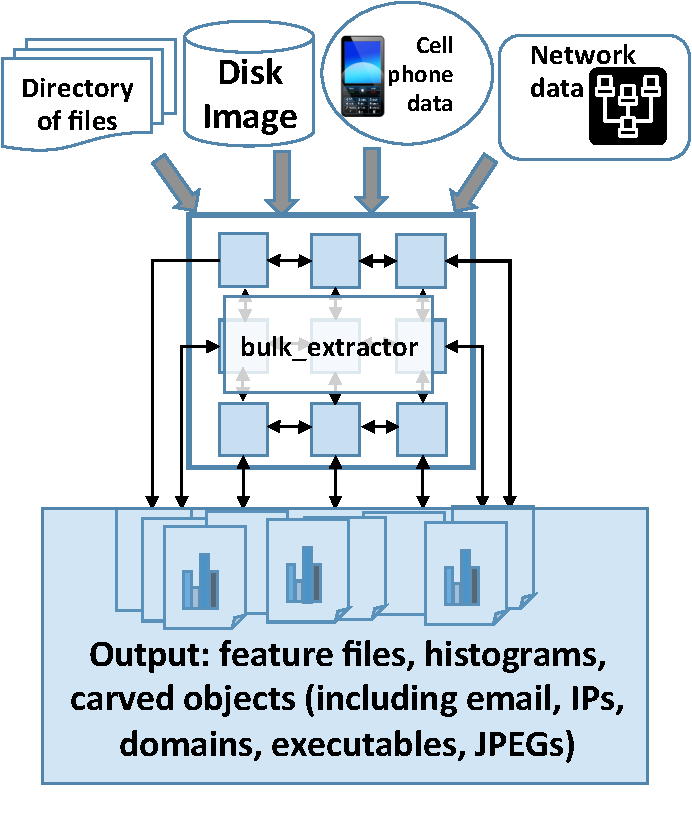
\includegraphics[scale=.6]{highLevelBulk}
  \captionof{figure}{\bulk extracts information from digital evidence}
  \label{fig:highLevelBulk}
\end{center}
\noindent
This fact sheet provides a brief introduction to \bulk including its applications, how it works, a brief description of how to operate it and how it can be expanded. More detailed information about \bulk can be found in two separate documents, the \textbf{\bulk Users Manual}\cite{usersManual} and the \textbf{\bulk Programmers Manual for Developing Plug-ins}\cite{programmersManual}. 

\section*{What is it good for?}
\bulk can be useful for many applications including digital media triage, examining digital media and extracting information for an automated pipeline.  It is a useful forensic investigation tool for many tasks such as malware and intrusion investigations, identity investigations and cyber investigations, as well as analyzing imagery and password cracking.

\subsubsection*{Forensic Investigation Tool}
\bulk is an efficient tool for many types of forensic investigations. Figure~\ref{fig:investigationTypes} shows some of those investigation types and lists the features found by \bulk. For example, \bulk will find ELF executables, Windows Prefetch files, Windows Executables and JSON information; all of these features can be useful for malware and intrusion investigations. The figure also shows the names of the feature files that \bulk produces containing the relevant information. For example, AES keys are stored in \texttt{aes.txt}.
\begin{center}
	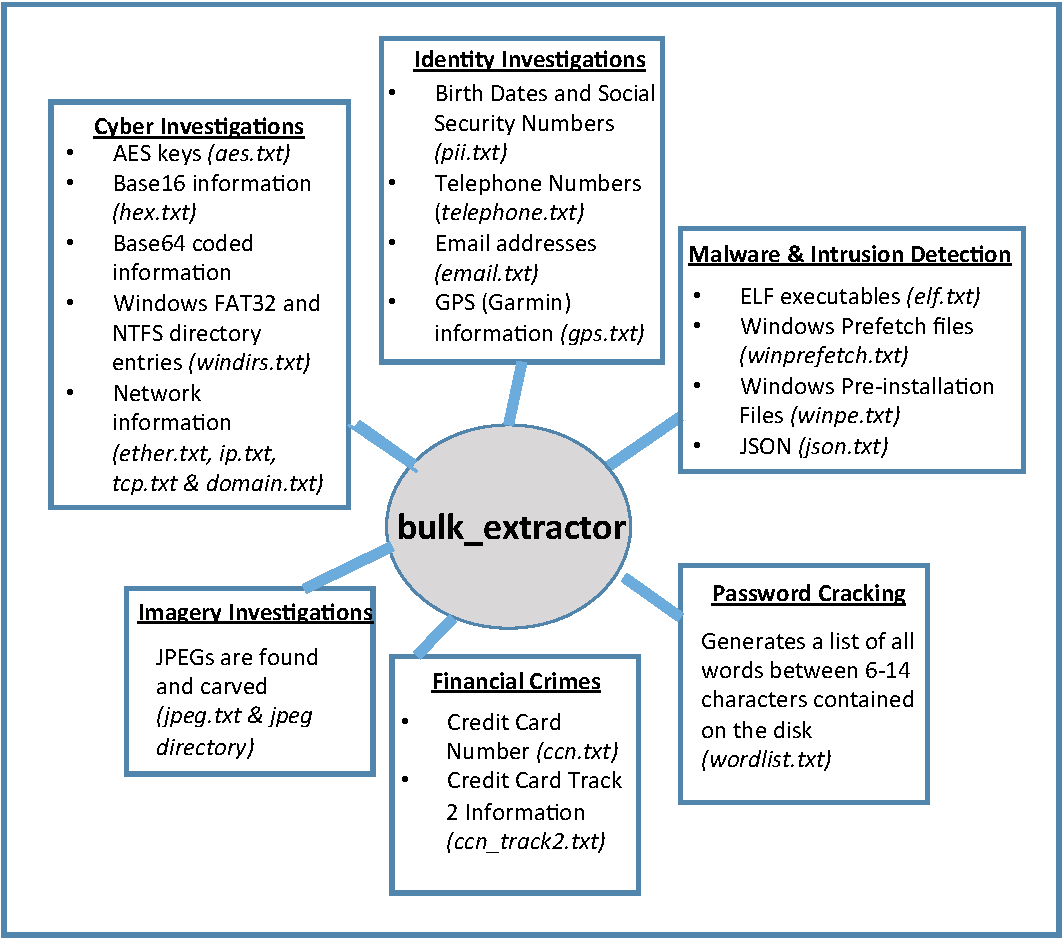
\includegraphics[scale=.80]{investigationTypes}
	\captionof{figure}{Some of the types of investigations \bulk supports}
	\label{fig:investigationTypes}
\end{center}

\subsubsection*{Digital Media Triage}
Digital media triage is a rapid and automated analysis process where investigators determine the immediate investigative value of a specific piece of digital media. Digital media triage answers the essential, time-critical questions: \textit{Will this digital media add value to my investigation?} and \textit{Should I perform an in-depth analysis of this media?} \\

\noindent
\bulk performs bulk data analysis, rapidly processing digital media and extracting salient features. For example, using \bulk  investigators can determine which laptop or telephone has the largest collection of credit card numbers, allowing investigators to choose which disk to analyze first. It can identify which hard drives or cell phones contain email addresses of interest. \bulk can even generate new leads, without the need for in-depth media analysis\cite{digitalMediaTriage}.


\subsubsection*{Examining Digital Media}
\bulk allows users to browse and search digital media. The output produced after running \bulk on a digital artifact includes a multitude of information including features, histograms of features and carved objects. For example:
\begin{itemize}
\item Features are grouped by feature type (e.g. all email addresses in one file, IP addresses in another). Features are shown in context and appear in the feature file in the order they occur on the disk. 
\item Users can utilize post-processing tools provided with \bulk to find the exact file in which a feature is found.  For example, given an email header feature, the post-processing tool can point the user to the complete email.
\item Features are extracted from compressed and encoded data. Users can see information that is not otherwise human read-able in it's existing digital format. 
\item Histogram files show the features found, grouped by type and sorted by frequency of occurrence. Users can look at the email histogram file to browse the email addresses, seeing those that occur most frequently first.
\item Carved objects are placed in folders in the output directory and can be viewed by users. For example, Figure~\ref{fig:carvedJPEG} was found encoded in GZIP format on a disk image from the M57 Patents Scenario (\url{http://digitalcorpora.org/corpora/scenarios/m57-patents-scenario} in GZIP format and carved by \bulk. The carving capability provided by \bulk allows users to browse JPEG, RAR and ZIP files found on the disk image that they might not otherwise be able to access or view.
\end{itemize}
Through its output, \bulk provides a means for users to browse the information contained within digital media.
\begin{center}
	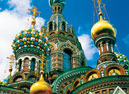
\includegraphics[scale=.80]{carvedJPEG.jpg}
	\captionof{figure}{A JPEG carved from GZIP encoded data on the M57 Patents Scenario disk image}
	\label{fig:carvedJPEG}
\end{center}

\subsubsection*{Information for an Automated Pipeline}
Intelligence analysts are inundated with an overabundance of digital information that requires analysis. That information is usually processed in some sort of automated (often real-time) pipeline. \bulk can be used to extract information from the automated pipeline. It can operate on digital information extracted from a data stream, including network data. It can be operated solely from the command line, making it easy to link it into an automated pipeline of incoming information. 

\section*{How does it work?}
\bulk takes in input data, divides it into equal sized buffers and passes the buffers to different scanners for processing; the scanners write the output which includes feature files, histogram files and carved objects. The scanners in \bulk extract many different types of features including: \textbf{AES keys, credit card numbers, credit card track 2 information, internet domains, Executable and Linkable Format (ELF), email addresses, ethernet MAC addresses, EXIFs from JPEGs and video segments, GPS coordinates, hex encoded data, IP addresses, carved JPEG files, JSON files and objects, carved KML files, carved RAR files, TCP information, telephone numbers, URLs (including Facebook, Microsoft Live, search terms and services), vCard data, Windows FAT32 and NTFS directory entries, Windows Portable executables, Windows Prefetch files} and \textbf{ZIP files}. \\

\noindent
Feature files are written using the feature recording system. As features are discovered by a scanner, they are sent to the feature recorder and recorded in the appropriate file. Multiple scanners might write to the same feature file. For example, the \textbf{\textit{exif}} scanner searches the file formats used by digital cameras and finds GPS coordinate in images. Those finding are written to the output file \texttt{gps.txt} by the \textit{\textbf{gps}} feature recorder. A separate scanner, the \textbf{\textit{gps}} scanner, searches Garmin Trackpoint data and finds GPS coordinates, also writing them to \texttt{gps.txt}. Some scanners write to several feature files. For example, the \textbf{\textit{email}} scanner looks for email addresses, domains, URLs and RFC822 headers and writes them to \texttt{email.txt}, \texttt{domain.txt}, \texttt{url.txt}, \texttt{rfc822.txt} and \texttt{ether.txt} respectively. \\

\noindent
The multitude of scanners within \bulk each serve a different function and work in parallel to decompress, extract and carve information from the data. Scanner functions include:
\begin{itemize}
\item Finding specific features in the data (like email addresses , credit card numbers, phone numbers and social security numbers)
\item Decompressing compressed data buffers to create more buffers. For example, the GZIP scanner decompresses GZIP'd data and creates newly decompressed buffers that are sent to other scanners for feature extraction.
\item Carving specific types of data. Currently, \bulk scanners provide carving of contiguous JPEG, ZIP and RAR files. 
\end{itemize}
Table ~\ref{tab:inputdata} shows many of the scanners in \bulk v1.4 and the data type on which each operates. The table also shows many of the data types that are scanned for features but may not appear specifically in a feature file.  For example, the \textbf{\textit{hiber}} scanner decompresses Windows Hibernation files and then sends the decompressed fragments to other scanners for feature extraction. HIBER information only appears in feature files to indicate if a feature, such as an email address, was found in HIBER compressed data. \\
\begin{table}[!ht]
%use [H] if you want to force table into a specific place (depending on final edits)
\centering
\caption{Input Data Processed by the Scanners}
\label{tab:inputdata}
\begin{tabular}{|p{2.5 cm}|p{12 cm}|}
\hline \hline
\center{\textbf{Scanner Name}} & \center{\textbf{Data Type}} \tabularnewline
\hline
\textbf{\textit{base16}} & Base 16 (hex) encoded data (includes MD5 codes embedded in the data)\\
\hline
\textbf{\textit{base64}} & Base 64 code\\
\hline
\textbf{\textit{elf}} & Executable and Linkable Format (ELF)\\
\hline
\textbf{\textit{exif}} & EXIF structures from JPEGS (and carving of JPEG files)\\
\hline
\textbf{\textit{gzip}} & GZIP files and ZLIB-compressed GZIP streams\\
\hline
\textbf{\textit{aes}} & In-memory AES keys from their key schedules\\
\hline
\textbf{\textit{json}} & JavaScript Object Notation files and objects downloaded from web servers, as well as JSON-like objects found in source code\\
\hline
\textbf{\textit{jpeg}} & JPEG carving. Default is only encoded JPEGs are carved. JPEGs without EXIFs are also carved\\
\hline
\textbf{\textit{kml}} & KML files (carved)\\
\hline
\textbf{\textit{rar}} &  RAR components in unencrypted archives are decrypted and processed. Encrypted RAR file are carved.\\
\hline
\textbf{\textit{pdf}} & Text from PDF files (extracted for processing not carved)\\
\hline
\textbf{\textit{windirs}} & Windows FAT32 and NTFS directory entries\\
\hline
\textbf{\textit{hiber}} & Windows Hibernation File Fragments (decompressed and processed, not carved)\\
\hline
\textbf{\textit{winprefetch}} & Windows Prefetch files, file fragments (processed)\\
\hline
\textbf{\textit{winpe}} & Windows Portable Executable (PE) files (.exe and .dll files notated with MD5 hash of first 4k)\\
\hline
\textbf{\textit{vcard}} & vCard files (carved)\\
\hline
\textbf{\textit{gps}} & XML from Garmin GPS devices (processed)\\
\hline
\textbf{\textit{zip}} & ZIP files and zlib streams (processed, and optionally carved)\\
\hline
\end{tabular}
\end{table}

\noindent
Histograms are a powerful tool for understanding certain kinds of evidence. \bulk creates histograms of several kinds of output features including but not limited to credit card numbers, domains, email addresses and URLs. A histogram of emails allows users to rapidly determine the drive's primary users,  the user's organization, primary correspondents and other email addresses. The feature recording system automatically creates histograms as data are processed. When the scanner writes to the feature recording system, the relevant histograms are automatically updated. 

\section*{How do I use it?}
\bulk is a command line tool with an accompanying graphical user interface tool, \textbf{Bulk Extractor Viewer}. All of the command line functionality of \bulk is also available in the \textbf{Bulk Extractor Viewer}. Users can access the functionality in whichever way they prefer. \\

\noindent
\bulk can be run on a Linux, MacOS or Windows system. The fastest way to run \bulk is using Linux on a Linux system. Another way to run \bulk faster is to run on a machine with more cores. \bulk is multi-threaded; running it on a computer with twice the number of cores typically makes it complete a run in half the time.  \\

\noindent
It is free and easy to install. Downloads are available at \url{http://www.digitalcorpora.org/downloads/bulk_extractor/}. The \textbf{\bulk Users Manual} \cite{usersManual} contains specific instructions, including a Quick Start guide, on how to get \bulk set up on your machine.

\section*{Can I expand it?}
Users can develop plug-ins, giving them the ability to expand \bulk to suit their needs. Plug-ins are external scanners that an individual or organization can run in addition to the open source capabilities provided with the \bulk system. The plug-in system gives the full power of \bulk to external developers, as all of \bulk's native scanners are written with the plug-in system. All of the scanners installed with \bulk use the plug-in system; in essence, \bulk is really just a framework for running plug-ins. The \textbf{Programmers Manual for Developing Scanner Plug-ins} \cite{programmersManual} provides specific details on how to develop and use plug-ins with \bulk.
%------------------------------------------------
\section*{Summary}
 To solve tomorrow's hard problems in automated computer forensics, we need systems built with open architectures that can rapidly integrate new technology and cutting edge research. \bulk is a powerful tool for digital forensics analysis that does just that.  It is freely available to interested users from \url{http://www.digitalcorpora.org/downloads/bulk_extractor}. 

%----------------------------------------------------------------------------------------
%	REFERENCE LIST
%----------------------------------------------------------------------------------------

\begin{thebibliography}{99} % Bibliography - this is intentionally simple in this template

\bibitem{Next10Years}
Garfinkel, Simson (2010).
\newblock Digital forensics research: the next 10 years
\newblock {\em Digital Investigation}, 7:S64-S73.

\bibitem{usersManual}
Bradley, Jessica and Garfinkel, Simson (2013).
\newblock \bulk Users Manual including Quick Start Guides
\newblock {\em http://digitalcorpora.org/downloads/bulk\_extract
or/doc/BEUsersManual.pdf}, 2013.

\bibitem{programmersManual}
Bradley, Jessica and Garfinkel, Simson (2013).
\newblock Programmers Manual for Developing Scanner Plug-ins
\newblock {\em http://digitalcorpora.org/downloads/bulk\_extract
or/doc/BEProgrammersManual.pdf}, July, 2013.	

\bibitem{digitalMediaTriage}
Garfinkel, Simson (2012).
\newblock Digital media triage with bulk data analysis and bulk\_extractor. 
\newblock{\em Computers and Security}, 32:56-72.

\bibitem{encodedEvidence}
Garfinkel, Simson and Nelson, Alex and White, Douglas and Roussev, Vassil (2010).
\newblock Using purpose-built functions and block hashes to enable small block and sub-file forensics
\newblock {\em Digital Investigation}, 7:S13-S23.

\end{thebibliography}

%----------------------------------------------------------------------------------------

\end{document}
